\documentclass[]{article}
\usepackage{geometry}[margin=1in]
\usepackage{amsmath}
\usepackage{physics}
\usepackage{graphicx}
\usepackage{cancel}
\usepackage{setspace}

\setlength\parindent{0pt}

\newcommand{\sectionname}{Section}

\setcounter{section}{-1}


%opening
\title{MECH 6300 - Problem Set C}
\author{Jonas Wagner}
\date{2020, October 23}



\begin{document}

\maketitle


\section{Inverted Pendulum System Introduction}

	\subsection{Design Application 2 Background}
	
		Design Application 2 is that of an inverted pendulum. This consists of a mass on a rod that extends upward from a movable cart that can be balanced at its upright equilibrium point.
		
		\begin{figure}[h]
			\centering
			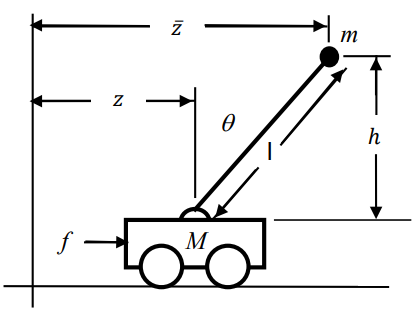
\includegraphics[width=0.5\linewidth]{Fig/DesignApplication2}
			\caption[]{Inverted Pendulum Mechanics Figure}
			\label{fig:designapplication2}
		\end{figure}
		
		Given the diagram, \figurename \ \ref{fig:designapplication2}, the following parameters are defined:
		\begin{align*}
			M &\equiv \text{Mass of the cart}\\
			m &\equiv \text{Mass at end of the rod}\\
			l &\equiv \text{Length of the rod}
		\end{align*}
		
		The two primary coordinates of the system are:
		\begin{align*}
			z &\equiv \text{Cart z-position}\\
			\theta &\equiv \text{Pendulum angle}
		\end{align*}
		
		Additional variables are defined in the figure:
		\begin{align*}
			h &\equiv \text{Mass height}\\
			\bar{z} &\equiv \text{Mass z-position}
		\end{align*} 
		
		These variables can be related to the primary coordinates as such:
		\begin{align}
			h		&= l \cos(\theta) \label{eq:h_def}\\
			\bar{z} &= z + l \sin(\theta) \label{eq:z_def}	
		\end{align}
		
		The derivatives of each of these variables can also be computed as such:
		\begin{align}
			\dot{h} &= -l \dot{\theta} \sin(\theta) \label{eq:h_dot}\\
			\dot{\bar{z}} &= \dot{z} + l \dot{\theta}\cos(\theta) \label{eq:z}
		\end{align}
		
		The total kinetic energy, $E_k$, can be defined as the sum of the kinetic energy of the cart and pendulum mass:
		\begin{align}
			E_k &= \frac{1}{2} M \dot{z}^2 + \frac{1}{2} m \qty(\sqrt{\dot{\bar{z}}^2 + \dot{h}^2})^2 \label{eq:E_k_original}\\
				&= \frac{1}{2} M \dot{z}^2 + \frac{1}{2} m \qty(\qty(\dot{z} + l \dot{\theta}\cos(\theta))^2 + \qty(-l \dot{\theta} \sin(\theta))^2)\nonumber\\
				&= \frac{1}{2} M \dot{z}^2 + \frac{1}{2} m \qty(\qty(\dot{z}^2 + 2 l \dot{z} \dot{\theta}\cos(\theta) + l^2 \dot{\theta}^2 \cos[2](\theta)) + \qty(l^2 \dot{\theta}^2 \sin[2](\theta)))\nonumber\\
				&= \frac{1}{2} M \dot{z}^2 + \frac{1}{2} m \qty(\dot{z}^2 + 2 l \dot{z} \dot{\theta}\cos(\theta) + l^2 \dot{\theta}^2 \qty(\cos[2](\theta)\sin[2](\theta)))\nonumber
		\end{align}
		
		This results in a simplified kinetic energy equation of:
		\begin{equation}
				E_k = \frac{1}{2} (M + m) \dot{z}^2 + m l \dot{z} \dot{\theta}\cos(\theta) + \frac{1}{2} l^2 \dot{\theta}^2
				\label{eq:E_k_simplified}
		\end{equation}
		
		The potential energy, $E_p$, consists only of the gravitational potential energy within the pendulum mass:
		\begin{align}
			E_p &= m g h\\
			E_p &= m g l \cos(\theta) \label{eq:E_p}
		\end{align}
		
		The Lagrangian can then be defined by the difference between the total kinetic \eqref{eq:E_k_simplified} and potential \eqref{eq:E_p} energy as follows:
		\begin{align}
			L &= E_k - E_p\\
			L &= \frac{1}{2} (M + m) \dot{z}^2 + m l \dot{z} \dot{\theta}\cos(\theta) + \frac{1}{2} ml^2 \dot{\theta}^2 - m g l \cos(\theta) \label{eq:L}
		\end{align}
	
	\subsection{$z$-coordinate Lagrange Equation}
	
		Utilizing the Lagrangian of the inverted pendulum system \eqref{eq:L}, the Z-coordinate Lagrange equation can be found using the following equation:
		\begin{equation}
			\dv{t} \qty(\pdv{L}{\dot{z}}) - \pdv{L}{z} = f
			\label{eq:lagrange_Z_original}
		\end{equation}
		
		First, the partial derivatives can be calculated as follows:
		\begin{align}
			\pdv{L}{\dot{z}} &= (M+m)\dot{z} + m l \dot{\theta}\cos(\theta) \label{eq:pdv_L_z_dot}\\
			\pdv{L}{z} &= 0 \label{eq:pdv_L_z}
		\end{align}
		
		The time derivative can then be computed from \eqref{eq:pdv_L_z_dot}:
		\begin{equation}
			\dv{t} \qty(\pdv{L}{\dot{z}}) = (M+m)\ddot{z} + m l \qty(\ddot{\theta}\cos(\theta) - \dot{\theta}^2\sin(\theta))
			\label{eq:dv_pdv_L_z_dot}
		\end{equation}
		
		The Lagrange equation can then be derived using \eqref{eq:lagrange_Z_original}, \eqref{eq:pdv_L_z}, and \eqref{eq:dv_pdv_L_z_dot}:
		\begin{equation}
			(M+m)\ddot{z} + m l \qty(\ddot{\theta}\cos(\theta) - \dot{\theta}^2\sin(\theta)) = f
			\label{eq:lagrange_Z}
		\end{equation}
	
	\subsection{$\theta$-coordinate Lagrange Equation}
	
		Utilizing the Lagrangian of the inverted pendulum system \eqref{eq:L}, the $\theta$-coordinate Lagrange equation can be found using the following equation:
		\begin{equation}
			\dv{t} \qty(\pdv{L}{\dot{\theta}}) - \pdv{L}{\theta} = 0
			\label{eq:lagrange_theta_original}
		\end{equation}
		
		First, the partial derivatives can be calculated as follows:
		\begin{align}
			\pdv{L}{\dot{\theta}} &= m l \dot{z} \cos(\theta) + m l^2 \dot{\theta} \label{eq:pdv_L_theta_dot}\\
			\pdv{L}{\theta} &= - m l \dot{z} \dot{\theta} \sin(\theta) + m g l \sin(\theta) \label{eq:pdv_L_theta}
		\end{align}
		
		The time derivative can then be computed from \eqref{eq:pdv_L_theta_dot}:
		\begin{equation}
			\dv{t} \qty(\pdv{L}{\dot{\theta}}) = m l^2 \ddot{\theta} + m l \ddot{z} \cos(\theta) - m l \dot{z} \dot{\theta} \sin(\theta)
			\label{eq:dv_pdv_L_theta_dot}
		\end{equation}
		
		The Lagrange equation can then be derived using \eqref{eq:lagrange_theta_original}, \eqref{eq:pdv_L_theta}, and \eqref{eq:dv_pdv_L_theta_dot}:
		\begin{align}
			 \qty(m l^2 \ddot{\theta} + m l \ddot{z} \cos(\theta) - m l \dot{z} \dot{\theta} \sin(\theta)) - \qty(- m l \dot{z} \dot{\theta} \sin(\theta) + m g l \sin(\theta))= 0 \nonumber\\
			 m l^2 \ddot{\theta} - m g l \sin(\theta) + m l \ddot{z} \cos(\theta) = 0
			\label{eq:lagrange_theta}
		\end{align}

	\subsection{Non-linear Equations of Motion:}
	
		The two Lagrange equations computed were computed in \eqref{eq:lagrange_Z} and \eqref{eq:lagrange_theta}:
		\begin{align}
			(M+m)\ddot{z} + m l \qty(\ddot{\theta}\cos(\theta) - \dot{\theta}^2\sin(\theta)) &= f  \tag{\ref{eq:lagrange_Z}}\\
			m l^2 \ddot{\theta} - m g l \sin(\theta) + m l \ddot{z} \cos(\theta) &= 0
			\tag{\ref{eq:lagrange_theta}}
		\end{align}

	\subsection{Linearized Model}
		Derive a linearized model at the upright equilibrium point using the following approximations:
		\begin{align*}
			\cos(\theta) 	&\approx 1\\
			\sin(\theta) 	&\approx \theta\\
			\dot{z}^2		&\approx 0\\
			\dot{\theta}^2  &\approx 0
		\end{align*}
		
			From \eqref{eq:lagrange_Z}, the following can be derived:
			\begin{align}
				(M+m)\ddot{z} &= f -ml \qty(\ddot{\theta}\cancelto{1}{\cos{\theta}} - \cancelto{0}{\dot{z}^2}\cancelto{\theta}{\sin{\theta}} ) \nonumber\\
				\ddot{z} &= \frac{f -ml \ddot{\theta}}{M+m} \label{eq:z_lin_init}
			\end{align}
		
			From \eqref{eq:lagrange_theta}, the following can be derived:
			\begin{align}
				m l^2 \ddot{\theta} &= m g l \cancelto{\theta}{\sin{\theta}} - m l \ddot{z} \cancelto{1}{\cos{\theta}} \nonumber\\
				\ddot{\theta} &= \frac{g\theta -\ddot{z}}{l} \label{eq:theta_lin_init}
			\end{align}
			
			By substituting \eqref{eq:theta_lin_init} into \eqref{eq:z_lin_init}, the following can be obtained:
			\begin{align}
				\ddot{z} &= \frac{f -m\bcancel{l} \qty(\cfrac{g\theta-\ddot{z}}{\bcancel{l}})}{M+m} \nonumber\\
				\ddot{z} \qty(1-\frac{m}{M+m}) &= \frac{f - mg\theta}{M+m} \nonumber\\
				\ddot{z} &= \frac{f-mg\theta}{\qty(1-\cfrac{m}{M+m}) \qty(M+m)} \nonumber\\
				\ddot{z} &= \frac{f-mg\theta}{M} \label{eq:z_lin}
			\end{align}
			
			\eqref{eq:theta_lin_init} can then rewritten as:
			\begin{align}
				\ddot{\theta} &= \frac{g\theta -\qty(\cfrac{f-mg\theta}{M})}{l} \nonumber\\
				\ddot{\theta} &= \frac{(m+M)g\theta - f}{Ml} \nonumber\\
				\ddot{\theta} &= \frac{(m+M)g\theta}{Ml} - \frac{f}{Ml} \label{eq:theta_lin}
			\end{align}

	\subsection{Standard State-Variable Format}
		Put the system into standard variable form:
		\begin{equation}
			\begin{aligned}
				\dot{\vb*{x}} &= A \vb*{x} + B \vb*{u}\\
				\vb*{y} &= C \vb*{x} + D \vb*{u}
			\end{aligned} \label{eq:state_eq_def}
		\end{equation}
		
		where $\vb*{x}$ is the following state vector:
		\begin{equation}
			\vb*{x} = \mqty[z \\ \dot{z} \\ \theta \\ \dot{\theta}] \label{eq:state_var}
		\end{equation}
	
		the output $\vb*{y}$ is defined as:
		
		\begin{equation}
			\vb*{y} = \mqty[z \\ \theta]
		\end{equation}
		
		and the input $\vb*{u}$ is defined as:
		\begin{equation}
			\vb*{u} = f
		\end{equation}
		
		The state-equations and  linearized equations \eqref{eq:z_lin} and \eqref{eq:theta_lin} can be used to generate the following state-variable equations:
		\begin{equation}
			\begin{aligned}
				\dot{z} &= \vb*{x}[2]\\
				\ddot{z} & = \frac{-mg}{M}\vb*{x}[3] + \frac{1}{M} \vb*{u}[1]\\
				\dot{\theta} & = \vb*{x}[4]\\
				\ddot{\theta} & = \frac{(m+M)g}{Ml}\vb*{x}[3] - \frac{1}{Ml} \vb*{u}[1]\\
				\\
				\vb*{y}[1] &= z = \vb*{x}[1]\\
				\vb*{y}[2] &= \theta = \vb*{x}[3]
			\end{aligned}
			\label{eq:state_eq_init}
		\end{equation}
		
		From the state-equations \eqref{eq:state_eq_init}, the following state-matrices can be derived:
		\setstretch{1.2}
		\begin{equation}
			\begin{aligned}
				&A = \mqty[	0 & 1 & 0 & 0\\
							0 & 0 & \cfrac{-mg}{M} & 0\\
							0 & 0 & 0 & 1\\
							0 & 0 & \cfrac{(m+M)g}{Ml}	& 0]
				&B = \mqty[	0\\
							\cfrac{1}{M}\\
							0\\
							\cfrac{-1}{Ml}] \\ \\
				&C = \mqty[	1 & 0 & 0 & 0\\
							0 & 0 & 1 & 0]
				&D = 0
			\end{aligned}
			\label{eq:state_matrices}
		\end{equation}
		\setstretch{1}
	
	\subsection{Design Application 1 Background}
		Design Application 1 describes a DC motor with a load. The system consists of a DC motor with an inertial load, $J$, that converts a voltage input, $e$, into a radial position, $\theta$.
		
		\begin{figure}[h]
			\centering
			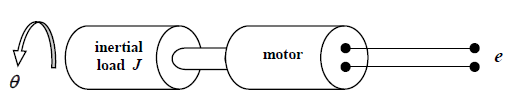
\includegraphics[width=0.7\linewidth]{Fig/DesignApplication1}
			\caption{DC Motor with Load Diagram}
			\label{fig:designapplication1}
		\end{figure}
		
		The following parameters are defined to describe the DC motor and load operation:
		\begin{align*}
			J &\equiv \text{Inertial Load}\\
			R &\equiv \text{Armature Resistance}\\
			K_1 &\equiv \text{Torque-Current Motor Constant}\\
			K_2 &\equiv \text{Voltage-Speed Motor Constant}
		\end{align*}
		
		The two primary State variables are defined as:
		\begin{align*}
			e &\equiv \text{Voltage Input}\\
			\theta &\equiv \text{Radial Position}
		\end{align*}
		
		Additional variables are defined as:
		\begin{align*}
			\tau 	&\equiv \text{Torque}\\
			i		&\equiv \text{Input Current}\\
			v 		&\equiv \text{Back EMF Voltage}\\
			\omega	&\equiv \text{Output Rotational Velocity}
		\end{align*}
		
		Given the physics of a DC brushed motor, the following relationships exist:
		\begin{align}
			\tau &= K_1 i \label{eq:tau_i_rel}\\
			v &= K_2 \omega \label{eq:v_omega_rel}\\
		\end{align}
		
		Additionally, with the assumption of 100\% \ efficiency, the following can be stated:
		\begin{align}
			k = K_1 &= K_2 \label{eq:K1_K2}
		\end{align}
		
		From Ohm's Law, the following is known:
		\begin{align}
			e - v &= Ri \nonumber\\
			i &= \frac{e-v}{R} \label{eq:armature_Ohms}
		\end{align}
		
		From rotational dynamics it is also known that:
		\begin{align}
			\tau &= J \dot{\omega} \label{eq:tau_omega_rel}\\
			\dot{\theta} &= \omega \label{eq:omega_def}
		\end{align}
		
		By equating \eqref{eq:tau_i_rel} and \eqref{eq:tau_omega_rel}, and then substituting \eqref{eq:armature_Ohms} and \eqref{eq:v_omega_rel}, the following can be derived:
		\begin{align}
			 J \dot{\omega}	&= \tau = K_1 i \nonumber\\
			 J \dot{\omega}	&= K_1 \qty(\frac{e-v}{R}) \nonumber\\
			 J \dot{\omega}	&= \frac{K_1 \qty(e - \qty(K_2 \omega))}{R} \nonumber\\
			 \dot{\omega}	&= \frac{K_1}{JR} e - \frac{K_1 K_2}{JR} \omega \label{eq:omega_state_eq}
		\end{align}
		
		The two state equations, \eqref{eq:omega_def} and \eqref{eq:omega_state_eq}, can then be rewritten in the standard state variable format:
		\begin{align}
			\mqty[	\dot{\theta}\\
					\dot{\omega}]
					&= \mqty[	0	&1\\
								0	&-\frac{K_1 K_2}{J R}]
						\mqty[	\theta\\
								\omega]
						+ \mqty[0\\
								\frac{K_1}{J R}] e \label{eq:DesignApp2_state_eq}
		\end{align}
	
	\subsection{Implementation Into Cart}\label{sec:p4_2}
		The electric motor can be introduced into the inverted pendulum cart by relating the output torque to the force excreted at the wheels.
		
		The relationships between rotational and linear movement are defined as:
		\begin{align}
			z &= r \theta \label{eq:z_theta_rel}\\
			\dot{z} &= r \omega \label{eq:zdot_omega_rel}\\
			f &= \frac{\tau}{r} \label{eq:f_tau_rel}
		\end{align}
		where $r$ is the radius of the wheel.
		
		Using the primary state equation for the DC motor, \eqref{eq:omega_state_eq}, torque output from the motor can be derived as:
		\begin{align}
			\tau &= J \dot{\omega} = \frac{K_1}{R} e - \frac{K_1 K_2}{R} \omega \label{eq:torque_eq}
		\end{align}
		
		Using the assumption \eqref{eq:K1_K2} and the relationships \eqref{eq:z_theta_rel}, \eqref{eq:zdot_omega_rel}, and \eqref{eq:f_tau_rel}, \eqref{eq:torque_eq} can be converted to the linear equivalent:
		\begin{align}
			f r &= \frac{k}{R} e - \frac{k^2}{R} \frac{\dot{z}}{r} \nonumber\\
			f &= \frac{k}{R r} e - \frac{k^2}{r^2} \dot{z} \label{eq:f_def}
		\end{align}
		
		This can then be substituted into \eqref{eq:z_lin} and \eqref{eq:theta_lin} to create the overall system equations of motion:
		\begin{align}
			\ddot{z} &= - \frac{mg}{M} \theta + \frac{1}{M} \qty(\frac{k}{Rr}e - \frac{k^2}{R r^2} \dot{z}) \label{eq:z_pend_eq}\\
			\ddot{\theta} &= \frac{(M+m)g}{M l} \theta - \frac{1}{M l} \qty(\frac{k}{R r} e - \frac{k^2}{R r^2}\dot{z}) \label{eq:theta_pend_eq}
		\end{align}
	
		These new equations of motion can then be adapted to the standard state-space representation as described in \eqref{eq:state_eq_def} as shown:
		\setstretch{1.2}
		\begin{equation}
			\begin{aligned}
				&A = \mqty[	0 & 1 					& 0 					& 0\\
							0 & \cfrac{-k^2}{MRr^2}	& \cfrac{-mg}{M} 		& 0 \\
							0 & 0 					& 0 					& 1\\
							0 & \cfrac{k^2}{MlRr^2}	& \cfrac{(m+M)g}{Ml}	& 0	]
				&B = \mqty[	0\\
							\cfrac{k}{MRr}\\
							0\\
							\cfrac{-k}{MlRr}] \\ &&\\
				&C = \mqty[	1 & 0 & 0 & 0\\
							0 & 0 & 1 & 0]
				&D = 0
			\end{aligned}
			\label{eq:pendulum_state_matrices}
		\end{equation}
		\setstretch{1}
	
	\subsection{Numerical Implementation}
		\subsubsection{State-Variable Descriptions}
			A numerical state variable description of the system can be calculated using the state-matricies from \eqref{eq:state_matrices} and substituting in the following numerical parameters:
			\begin{align*}
				&m = 0.2 \ \text{kg} \\
				&M = 1.0 \ \text{kg} \\
				&l = 1.0 \ \text{m} \\
				&g = 9.8 \ \text{m/s\textsuperscript{2}} \\
				&k = 2.0 \ \text{v-s} \\
				&R = 50  \ \Omega \\
				&r = 0.1 \ \text{m}
			\end{align*}
			
			The numerical state-variable description is calculated to be:
			\begin{equation}
				\begin{aligned}
					&A = \mqty[	0 & 1 	& 0 	& 0\\
								0 & -8	& -1.96 & 0 \\
								0 & 0	& 0 	& 1\\
								0 & -8	& 11.76	& 0	]
					&B = \mqty[	0\\
								0.4\\
								0\\
								-0.4] \\ && \\
					&C = \mqty[	1 & 0 & 0 & 0\\
								0 & 0 & 1 & 0]
					&D = 0
				\end{aligned}
				\label{eq:pendulum_state_matrices}
			\end{equation}
	
		\subsubsection{State Transition Matrix}
			The state transition matrix, $e^{At}$, is a very important matrix for modeling dynamical systems. The equivalent in the Laplace domain formed from state-space matrices is computed as $(sI - A)^{-1}$:
			
			\setstretch{1.5}
			\begin{equation}
				\begin{aligned}
					&(sI - A)^{-1} = \cfrac{1}{s (s-3.62) (s + 3.95) (s + 7.67)} \\
					&\ *\mqty[	(s - 3.62) (s + 3.95) (s + 7.67)	&(s - 3.43) (s + 3.43)		&-1.96 s			&-1.96\\
								0									&s (s - 3.43) (s + 3.43)	&-1.96 s^2			&-1.95 s\\
								0									&-8 s						&s^2 (s+8)			&s (s+8)\\
								0									&-8 s^2						&11.76 s (s+9.33)	&s^2 (s+8)
					]
				\end{aligned}
				\label{eq:pendulum_(sI-A)-1}
			\end{equation}
			\setstretch{1}
		
		\subsubsection{Transfer Function Calculation}
			The transfer functions of a state-space system can be calculated using the following equation:
			\begin{equation}
				H(s) = C (sI-A)^{-1} B + D
				\label{eq:tf_def}
			\end{equation}
			
			For the state-space model calculated for the Inverted Pendulum system, \eqref{eq:pendulum_state_matrices}, the Transfer Function matrix is defined as:
			
			\setstretch{1.5}
			\begin{equation}
				H(s) = \mqty[	\cfrac{0.4 \ (s^2 - 9.8)}{s \ (s^3 + 8s^2 - 11.76s - 109.76)}\\
								\cfrac{-0.4 \ s \ (s+16)}{s \ (s^3 + 8s^2 - 11.76s - 109.76}
								]
				\label{eq:pendulum_H(s)}
			\end{equation}
			\setstretch{1}
			
		\subsubsection{Stability of the System}
			The stability of any linear system can be determined by the roots of the characteristic polynomial. In the case of the inverted pendulum system, the characteristic polynomial is defined as:
			\begin{equation}
				\Delta (s) = s (s^3 + 8s^2 - 11.76s - 109.76) = s (s-3.62) (s + 3.95) (s + 7.67)
				\label{eq:pendulum_Delta(s)}
			\end{equation}
			
			This characteristic polynomial details that the is clearly unstable due to the root on the right-half plane: $(s-3.52)$

\newpage
\section{Problem 1: Various Measurement Observability}
	By redefining the output equation based on an arbitrary $C$ matrix, the observability of the inverted pendulum system can be determined for various measurement combinations.\\
	
	Let the state-space model be defined by the $A$ and $B$ matrices for the Inverted Pendulum system, \eqref{eq:pendulum_state_matrices}, and the redefined output equation:
	\begin{equation}
		y = C x \label{eq:generalOutputdef}
	\end{equation}
	
	The rank of the Observability Matrix defined as:
	\begin{equation}
		v = \mqty[C\\ CA\\ CA^2\\ CA^3] \label{eq:Vdef}
	\end{equation}
	
	can then be used to determine whether the pair $(C, A)$ is an observable pair.
	
	\subsection{Problem 1a - Cart Displacement Measurement Only}
		
		Let $C$ be defined as:
		\begin{equation}
			C_1 = \mqty[1	&0	&0	&0]
		\end{equation}
	
		The Observability matrix can then be calculated using \eqref{eq:Vdef}:
		\begin{equation}
			V_1 = \mqty[C\\ CA\\ CA^2\\ CA^3]
				= \mqty[1	&0	&0		&0\\
						0	&1	&0		&0\\
						0	&-8	&-1.96	&0\\
						0	&60	&15.68	&-1.96] \label{eq:v1def}
		\end{equation}
	
		Clearly, $\det(V_1) = 3.84 \neq 0$, as such $V_1$ is full rank. Thus, the system is fully observable when only measuring the cart displacement.
	
	\subsection{Problem 1b - Pendulum Angle Measurement Only}
		Let $C$ be defined as:
		\begin{equation}
			C_2 = \mqty[0	&0	&1	&0]
		\end{equation}
		
		The Observability matrix can then be calculated using \eqref{eq:Vdef}:
		\begin{equation}
			V_2 = \mqty[C\\ CA\\ CA^2\\ CA^3]
			= \mqty[0	&0	&1		&0\\
					0	&0	&0		&1\\
					0	&-8	&11.76	&0\\
					0	&64	&15.68	&11.76] \label{eq:v2def}
		\end{equation}
		
		Clearly, $\det(V_2) = 0$, as such $V_2$ is not full rank. Thus, the system is not fully observable when only measuring the pendulum angle.
	
	\subsection{Problem 1c - Cart Velocity Measurement Only}
		Let $C$ be defined as:
		\begin{equation}
			C_3 = \mqty[0	&1	&0	&0]
		\end{equation}
		
		The Observability matrix can then be calculated using \eqref{eq:Vdef}:
		\begin{equation}
			V_3 = \mqty[C\\ CA\\ CA^2\\ CA^3]
			= \mqty[0	&1		&0		&0\\
					0	&-8		&-1.96	&0\\
					0	&64		&15.68	&-1.96\\
					0	&-496	&-148	&15.68]\label{eq:v3def}
		\end{equation}
		
		Clearly, $\det(V_3) = 0$, as such $V_3$ is not full rank. Thus, the system is not fully observable when only measuring the cart velocity.
		
		
	\subsection{Problem 1d - Cart Velocity and Pendulum Angle measurement}
		Let $C$ be defined as:
		\begin{equation}
			C_4 = \mqty[0	&1	&0	&0\\
						0	&0	&1	&0]
		\end{equation}
		
		The Observability matrix can then be calculated using \eqref{eq:Vdef}:
		\begin{equation}
			V_4 = \mqty[C\\ CA\\ CA^2\\ CA^3]
				= \mqty[0	&1		&0		&0\\
						0	&0		&1		&0\\
						0	&-8		&-1.96	&0\\
						0	&0		&0		&1\\
						0	&64		&15.7	&-1.96\\
						0	&-8		&11.76	&0\\
						0	&-496	&-148.49&15.68\\
						0	&64		&15.68	&11.76] \label{eq:v4def}
		\end{equation}
		
		Since the entire first column of $V_4$ is zero, $V_4$ may not be full rank. Thus, the system is not fully observable when measuring the cart velocity and pendulum angle.
		
	
\newpage
\section{Problem 2}
	\subsection{Design Application 3 Background}
		Design Application 3 describes a system of two coupled carts. The system consists of two carts of mass $M_1$ and $M_2$ that are connected by a spring with constant $K$.
		
		\begin{figure}[h]
			\centering
			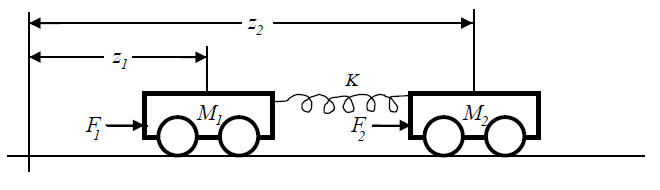
\includegraphics[width=0.7\linewidth]{Fig/DesignApplication3}
			\caption{Coupled Carts Figure}
			\label{fig:designapplication3}
		\end{figure}
		
		The following parameters are defined to describe the DC motor and load operation:
		\begin{align*}
			M_1 &\equiv \text{Mass of Cart 1}\\
			M_2 &\equiv \text{Mass of Cart 2}\\
			K &\equiv \text{Spring Constant}
		\end{align*}
		
		The two primary state variables are defined as:
		\begin{align*}
			z_1 &\equiv \text{Cart 1 Position}\\
			z_2 &\equiv \text{Cart 2 Position}
		\end{align*}
		
		The two inputs are defined as:
		\begin{align*}
			F_1 &\equiv \text{Cart 1 Force}\\
			F_2 &\equiv \text{Cart 2 Force}
		\end{align*}
		
		The Lagrangean of the system containing no potential energy is defined solely by the total kinetic energy:
		\begin{align}
			L &= \frac{1}{2} \qty(M_1 \dot{z_1}^2 + M_2 \dot{z_2}^2) \label{eq:carts_lagrange}
		\end{align}
		
		Additionally, the force on excreted by the spring on each cart is equal and opposite:
		\begin{align}
			F_s &= K(z_2 - z_1) = F_{s1} = F_{s2} \label{eq:spring_force}
		\end{align}
		
		The lagrangian equations for $z_1$ and $z_2$ can then be defined as:
		\begin{align}
			\dv{t}\qty(\pdv{L}{\dot{z_1}}) - \pdv{L}{z_1} &= F_1 + F_s \label{eq:carts_lagrange_eq1}\\
			\dv{t}\qty(\pdv{L}{\dot{z_2}}) - \pdv{L}{z_2} &= F_2 - F_s \label{eq:carts_lagrange_eq2}
		\end{align}	
		
		The dynamics can then be easily calculated from \eqref{eq:carts_lagrange_eq1} and \eqref{eq:carts_lagrange_eq2} as:
		\begin{align}
			M_1 \ddot{z_1} &= F_1 + K(z_2 - z_1) \label{eq:carts_state_eq1}\\
			M_2 \ddot{z_2} &= F_2 - K(z_2 - z_1) \label{eq:carts_state_eq2}
		\end{align}
		
	\subsection{Integration of Motors}
		Integration of motors into the coupled carts system can be done by relating the output torque of the motors to the force excreted by the wheels of each cart.\\
		
		First, the following parameters for the motors can be defined as:
		\begin{align*}
			k_i &\equiv \text{Motor Torque Constant}\\
			R_i &\equiv \text{Motor Armature Resistance}\\
			r_i &\equiv \text{Motor Tourque-Force Relationship}\\
		\end{align*}
		
		The following variables are also defined for each motor:
		\begin{align*}
			\tau_i &\equiv \text{Motor Output Torque}\\
			f_i &\equiv \text{Motor Output Force}\\
			e_i &\equiv \text{Motor Applied Voltage}
		\end{align*}
		
		From calculations done in \sectionname \ \ref{sec:p4_2}, specifically \eqref{eq:f_def}, it is known that for each motor:
		\begin{align}
			F_i &= \frac{k_i}{R_i r_i} e_i - \frac{k_i^2}{R_i r_i^2} \dot{z_i} \label{eq:carts_f_def}
		\end{align}

		
	\subsection{Cart Dynamics}
		The dynamics of the first cart can be described by substituting \eqref{eq:carts_f_def} into \eqref{eq:carts_state_eq1}:
		\begin{align}
			M_1 \ddot{z_1} &= \frac{k_1}{R_1 r_1} e_1 - \frac{k_1^2}{R_1 r_1^2} \dot{z_1} + K(z_2 - z_1) \nonumber\\
			\ddot{z_1} &= -\frac{K}{M_1} z_1 + \frac{K}{M_1} z_2 - \frac{k_1^2}{M_1 R_1 r_1^2} \dot{z_1} + \frac{k_1}{M_1 R_1 r_1} e_1
		\end{align}
	
		The dynamics of the second cart can be described by substituting \eqref{eq:carts_f_def} into \eqref{eq:carts_state_eq2}:
		\begin{align}
			M_2 \ddot{z_2} &= \frac{k_2}{R_2 r_2} e_2 - \frac{k_2^2}{R_2 r_2^2} \dot{z_2} - K(z_2 - z_1) \nonumber\\
			\ddot{z_2} &= \frac{K}{M_2} z_1 - \frac{K}{M_2} z_2 - \frac{k_2^2}{M_2 R_2 r_2^2} \dot{z_2} + \frac{k_2}{M_2 R_2 r_2} e_2
		\end{align}
	
		With the state vector, $x$, and input vector, $u$, defined as:
		\begin{align}
			x &= \mqty[z_1\\ z_2\\ \dot{z_1}\\ \dot{z_2}] \label{eq:carts_x_def}\\
			\nonumber\\
			u &= \mqty[e_1\\ e_2] \label{eq:carts_u_def}
		\end{align}
		
		the state equations can be defined as:
		\begin{equation}\label{eq:carts_state_eqs}
			\begin{aligned}
				\dot{x}[1] &= x[3]\\
				\dot{x}[2] &= x[4]\\
				\dot{x}[3] &= -\frac{K}{M_1} x[1] + \frac{K}{M_1} x[2] - \frac{k_1^2}{M_1 R_1 r_1^2} x[3] + \frac{k_1}{M_1 R_1 r_1} u[1]\\
				\dot{x}[4] &= \frac{K}{M_2} x[1] - \frac{K}{M_2} x[2] - \frac{k_2^2}{M_2 R_2 r_2^2} x[4] + \frac{k_2}{M_2 R_2 r_2} u[2]
			\end{aligned}
		\end{equation}

	\subsection{Output Equation}
		The output equation is a function of the state vector and is not directly dependent on the input. With the output vector, $y$, defined as:
		\setstretch{1.25}
		\begin{align}
			y &= \mqty[z_1\\ z_2]\label{eq:carts_y_def}
		\end{align}
		\setstretch{1}
		
		the output equations can be defined as:
		\begin{equation}\label{eq:carts_y_ouput_eqs}
			\begin{aligned}
				y[1] &= x[1]\\
				y[2] &= x[2]
			\end{aligned}
		\end{equation}
	
	\subsection{State-Space Matrix Formulation}
		The coupled carts system can be put in the standard state-space formulation:
		\begin{equation}\label{eq:state_space_eqs_def}
			\begin{aligned}
				\dot{x} &= A x + B u\\
				y &= C x + D u
			\end{aligned}
		\end{equation}
		 
		 by defining the state matrices based on \eqref{eq:carts_state_eqs} and \eqref{eq:carts_y_ouput_eqs}.
		 \begin{equation}
 			\begin{aligned}
		 		A = \mqty[	0	& 0			& 1					& 0\\
					 		0	& 0	 		& 0					& 1\\
					 		-\cfrac{K}{M_1}	& \cfrac{K}{M_1}	& -\cfrac{k_1^2}{M_1 R_1 r_1^2}	& 0\\
					 		\cfrac{K}{M_2}	& -\cfrac{K}{M_2}	& 0								& -\cfrac{k_2^2}{M_2 R_2 r_2^2}
					 		] \ \ \
		 		&B = \mqty[ 0						& 0\\
					 		0						& 0\\
					 		\cfrac{k_1}{M_1 R_1 r_1}	& 0\\
					 		0						& \cfrac{k_2}{M_2 R_2 r_2}
					 		]\\
		 		C = \mqty[\dmat[0]{1,1}] \ \ \
		 		&D = \mqty[\zmat{2}{2}]
		 	\end{aligned}
	 		\label{eq:carts_state_matrices}
		 \end{equation}
	
	\subsection{Numerical State-Variable Description}
		A numerical state variable description of the system can be calculated using the state-matricies from \eqref{eq:state_matrices} and substituting in the following numerical parameters:
		\begin{align*}
			M_1 = M_2 &= 1.0 \ \text{kg} \\
			K &= 40 \ \text{N/m}\\
			k &= 2.0 \ \text{v-s} \\
			R &= 100  \ \Omega \\
			r &= 0.01 \ \text{m}
		\end{align*}
	
		The numerical state space model can then be calculated as:
		 \begin{equation}
			\begin{aligned}
				A = \mqty[	0	& 0		& 1		& 0\\
							0	& 0	 	& 0		& 1\\
							-40	& 40	& -400	& 0\\
							40	& -40	& 0		& -400
							] \ \ \
				&B = \mqty[ 0	& 0\\
							0	& 0\\
							2	& 0\\
							0	& 2
							]\\
				C = \mqty[	1	&0	&0	&0\\
							0	&1	&0	&0] \ \ \
				&D = \mqty[\zmat{2}{2}]
			\end{aligned}
			\label{eq:carts_state_matrices}
		\end{equation}
		
		\subsubsection{Transfer Function Calculations}
			The transfer functions for the system can be directly calculated using \eqref{eq:tf_def}. For the dual cart system, the transfer function matrix can be calculated as:
			\begin{equation}
				H(s) = \mqty[	\cfrac{2}{s^2+400s+40}	&\cfrac{80}{(s^2+400s+40)^2}\\
								0						&\cfrac{2}{2^2+400s+40}
								]
			\end{equation}
	
		\subsubsection{System Pole Calculation}
			The characteristic equation for the dual cart system can be calculated with $\det(sI-A)$ and is defined as:
			\begin{equation}
				\Delta (s) = (s^2 + 400s +40)^2 = (s+0.1)^2(s+400)^2
				\label{eq:carts_Delta_s}
			\end{equation}
			
			From \eqref{eq:carts_Delta_s} it can be seen that the system poles and multiplicities are defined as:
			\begin{equation}
				\begin{aligned}
					&\lambda_1 = -0.1, \ m_1 = 2\\
					&\lambda_2 = -400, \ m_2 = 2
				\end{aligned}
			\end{equation}
		
			From these poles it can be seen that the carts are a stable and over-damped system.
	
	\newpage
	\subsection{Problem 2a - Single Motor Controlability Analysis}
		To test whether the system is fully controllable using only the first motor, the following can be redefined: $\frac{k_2}{M_2 R_2 r_r} = 0$. This results in the input matrix, $B$, to be redefined as:
		
		\begin{equation}
			B_1 = \mqty[0	&0\\
						0	&0\\
						2	&0\\
						0	&0]
		\end{equation}
		
		The controlability of the system pair $(A, B_1)$ can then be determined by analyzing the controllability matrix defined as:
		
		\begin{equation}
			\begin{aligned}
				U_1 &= \mqty[B		&A B_1		&A^2 B_1	&A^3 B_1]\\
					&= \mqty[0	&0	&2		&0	&-800	&0	&3.2e5	&0\\
							 0	&0	&0		&0	&0		&0	&80		&0\\
							 2	&0	&-800	&0	&3.2e5	&0	&-1.3e8	&0\\
							 0	&0	&0		&0	&80		&0	&-6.4e4	&0]
			\end{aligned}
		\end{equation}
		
		Clearly, given the 4 independent non-zero columns, it can be seen $\rank(U_1) = 4$. Thus, the system is fully controllable using a single motor.
		
	\subsection{Problem 2b - Both Motor Controlability Analysis}
		Although given the previous result, it can be determined that the system is controllable through inheritance, this can be confirmed by testing the system pair with both inputs as defined in \eqref{eq:carts_state_matrices}.
		
		The controlability of the system pair $(A, B)$ can then be determined by analyzing the controllability matrix defined as:
		
		\begin{equation}
			\begin{aligned}
				U_2 &= \mqty[B		&AB				&A^2B			&A^3B]\\
					&= \mqty[0	&0	&2		&0		&-800	&0		&3.2e5	&80\\
							 0	&0	&0		&2		&0		&-800	&80		&3.2e5\\
						 	 2	&0	&-800	&0	 	&3.2e5	&0		&-1.3e8	&-6.4e4\\
							 0	&2	&0		&-800	&80		&3.2e5	&-6.4e4	&-1.3e8]
			\end{aligned}
		\end{equation}
		
		It can also be determined that $\rank(U_2) = 4$. Thus, the system is fully controllable using both motors.
	
	\newpage
	\subsection{Problem 2c - One Cart Position Observability Analysis}
		To test whether the system is fully observable if only the position of the first cart is measured, a $C$ matrix can be defined as:
		
		\begin{equation}
			C_1 = \mqty[1	&0	&0	&0\\
					  	0	&0	&0	&0]
		\end{equation}

		The observability of the system pair $(A, C)$ can then be determined by analyzing the observability matrix defined as:
		
		\begin{equation}
			V_1 = \mqty[C_1\\ C_1A\\ C_1A^2\\ C_1A^3]
				= \mqty[1		&0		&0		&0\\
						0		&0		&0		&0\\
						0		&0		&1		&0\\
						0		&0		&0		&0\\
						-40		&40		&-400	&0\\
						0		&0		&0		&0\\
						16000	&-16000	&16000	&40\\
						0		&0		&0		&0]
		\end{equation}
		
		Clearly, $\rank(V_1) = 4$. Thus, the system is fully observable by measuring only the position of the first cart.

	\subsection{Problem 2d - One Cart Velocity Observability Analysis}
		To test whether the system is fully observable if only the velocity of the first cart is measured, a $C$ matrix can be defined as:
		
		\begin{equation}
			C_2 = \mqty[0	&0	&1	&0\\
						0	&0	&0	&0]
		\end{equation}
		
		The observability of the system pair $(A, C_2)$ can then be determined by analyzing the observability matrix defined as:
		
		\begin{equation}
			V_2 = \mqty[C_2\\ C_2A\\ C_2A^2\\ C_2A^3]
				= \mqty[0		&0		&1		&0\\
						0		&0		&0		&0\\
						-40		&40		&-400	&0\\
						0		&0		&0		&0\\
						16000	&-16000	&16000	&40\\
						0		&0		&0		&0\\
						-6.4e7	&6.4e7	&-6.4e7	&-3.2e4\\
						0		&0		&0		&0]
		\end{equation}
		
		In order to test the rank of $V_2$, the non-zero rows are complied into the following matrix:
		
		\begin{equation}
			\tilde{V_2} = \mqty[0		&0		&1		&0\\
								-40		&40		&-400	&0\\
								16000	&-16000	&16000	&40\\
								-6.4e7	&6.4e7	&-6.4e7	&-3.2e4]
		\end{equation}
		
		To test if $\tilde{V_2}$ is full rank, the determinant is taken: $\det(\tilde{V_2}) = 0$. Thus, $\tilde{V_2}$ is not full rank, and therefore, $\rank(V_2) < 4$. Thus, the system is not fully observable by measuring only the velocity of the first cart.
			
		\subsection{Problem 2d - One Cart Velocity Observability Analysis}
			To test whether the system is fully observable if only the velocities of the first and second cart are measured, a $C$ matrix can be defined as:
			
			\begin{equation}
				C_3 = \mqty[0	&0	&1	&0\\
							0	&0	&0	&1]
			\end{equation}
			
			The observability of the system pair $(A, C_3)$ can then be determined by analyzing the observability matrix defined as:
			
			\begin{equation}
				V_3 = \mqty[C_3\\ C_3A\\ C_3A^2\\ C_3A^3]
					= \mqty[0		&0		&1		&0\\
							0		&0		&0		&1\\
							-40		&40		&-400	&0\\
							40		&-40		&0		&-400\\
							16000	&-16000	&16000	&40\\
							-16000	&16000	&40		&16000\\
							-6.4e7	&6.4e7	&-6.4e7	&-3.2e4\\
							6.4e7	&-6.4e7	&-3.2e4	&-6.4e7]
			\end{equation}
			
			The rank of $V_3$ can be determined using the reduced-row echelon form given as:
			\begin{equation}
				\tilde{V_3} = \mqty[1	&-1	&10	&5e-3\\
									0	&0	&1	&1\\
									0	&0	&0	&1\\
									0	&0	&0	&0\\
									0	&0	&0	&0\\
									0	&0	&0	&0\\
									0	&0	&0	&0\\
									0	&0	&0	&0]
			\end{equation}
			
			Thus, $\rank(\tilde{V_2}) = 3$, and therefore, $\rank(V_2) < 4$. This leads to the conclusion that the system is not fully observable by measuring only the velocity of both the first and second cart.
		
\end{document}
